\subsection{Model-driven fitting methods}
\label{ch:proc_model}
When acquiring sensor data from physical objects it is often difficult or even impossible to analytically describe the resulting value, as there are numerous environmental factors influencing the signal and the properties of the object might not be clearly determined. Considering the human body, there is a mostly unconstrained number of sizes, shapes and biological properties that influence the response to an electric field. Thus, in order to fit sensor outputs to the potential object configurations, simplified models can be used that resemble the actual physical effects and can be described analytically. Regarding capacitance of the human body relative to a single sensor, a common abstraction is a sphere having a diameter close to the height of an average human \cite{seaver1997human}. Models based on a single geometric objects are considered single-body, while connected geometric objects that comprise a single model can be called multi-body. Smith used a model of multiple spheres to approximate arm position and rotation above an array of capacitive proximity sensors \cite{smith1998electric}. Another possibility is adapting the models to a derived physical effect. Harada et al. are using the projected pressure distribution of a virtual skeleton and body model on a flat surface to create a pressure distribution that can be compared to the actual pressure effect generated by an actual human body resting on a set of sensors \cite{harada2000human}. In this section I will describe two novel methods to fit abstracted models of the human body to sensor readings acquired from smart furniture systems. The first method uses a cylindrical human body model to match the posture of one or two bodies on a bed, the second method uses a multi-body skeleton that is fitted to sensor readings determining posture on a chair.
\subsubsection{Single-body models}
\begin{minipage}{\linewidth}
\centering
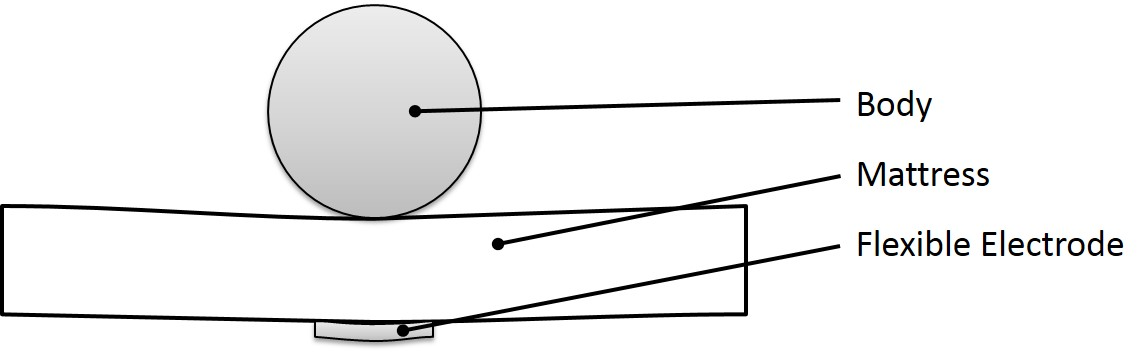
\includegraphics[width=0.8\textwidth]{images/proc_hetero_flexpressure}
\captionof{figure}{Object on mattress decreases distance and changes geometry of flexible electrode \cite{braun2012context}}
\label{fig:proc_hetero_flexpressure}
\end{minipage}

While models are more often applied directly to the capacitive sensor data, it is also possible to use a different property that is derived from it. Together with Henning Heggen, I developed a system that uses flexible electrodes that bend on pressure. In previous experiments we observed that bending a calibrated flexible electrode results in a higher value of the sensor. Thus, the idea was created to use this effect for combining presence and pressure detection. A first application was to use such a system on the slatted frame of a bed \cite{braun2012context}. The following section is based on two different publications \cite{Hamisu2010,braun2012context}. If an object is applying force to the mattress there are two cumulative effects. The object will be in detection range of the sensors, decreasing the distance by deforming the mattress and the applied pressure changes the geometry of the flexible electrode, resulting in a higher sensor value. The basic idea is shown in Figure \ref{fig:proc_hetero_flexpressure}. If a model is used that approaches the pressure distribution of a human body, a small number of capacitive proximity sensors equipped with flexible electrodes should allow to detect different posture and occupation configurations on the bed, including distinguishing sitting and lying, as well as one or two present persons. While the sensor values are increasing according to higher pressure, this relationship is highly non-linear and influenced by three groups of system parameters The sensor system parameters include the sensor design, e.g. excitation voltage and frequency, as well as geometry and material of the electrode. These parameters additionally determine range and precision of the overall system. The second group are environmental parameters that influence the conductivity of the excited electric field, including humidity and temperature. The third group are the bed parameters. These include the hardness of the slatted frame that influences the geometric deformation of the affixed electrodes and the mattress parameters, comprised of hardness, thickness, material and type, influencing how far the body is away from the electrodes and how the pressure is distributed onto the slatted frame.

\begin{minipage}{\linewidth}
\centering
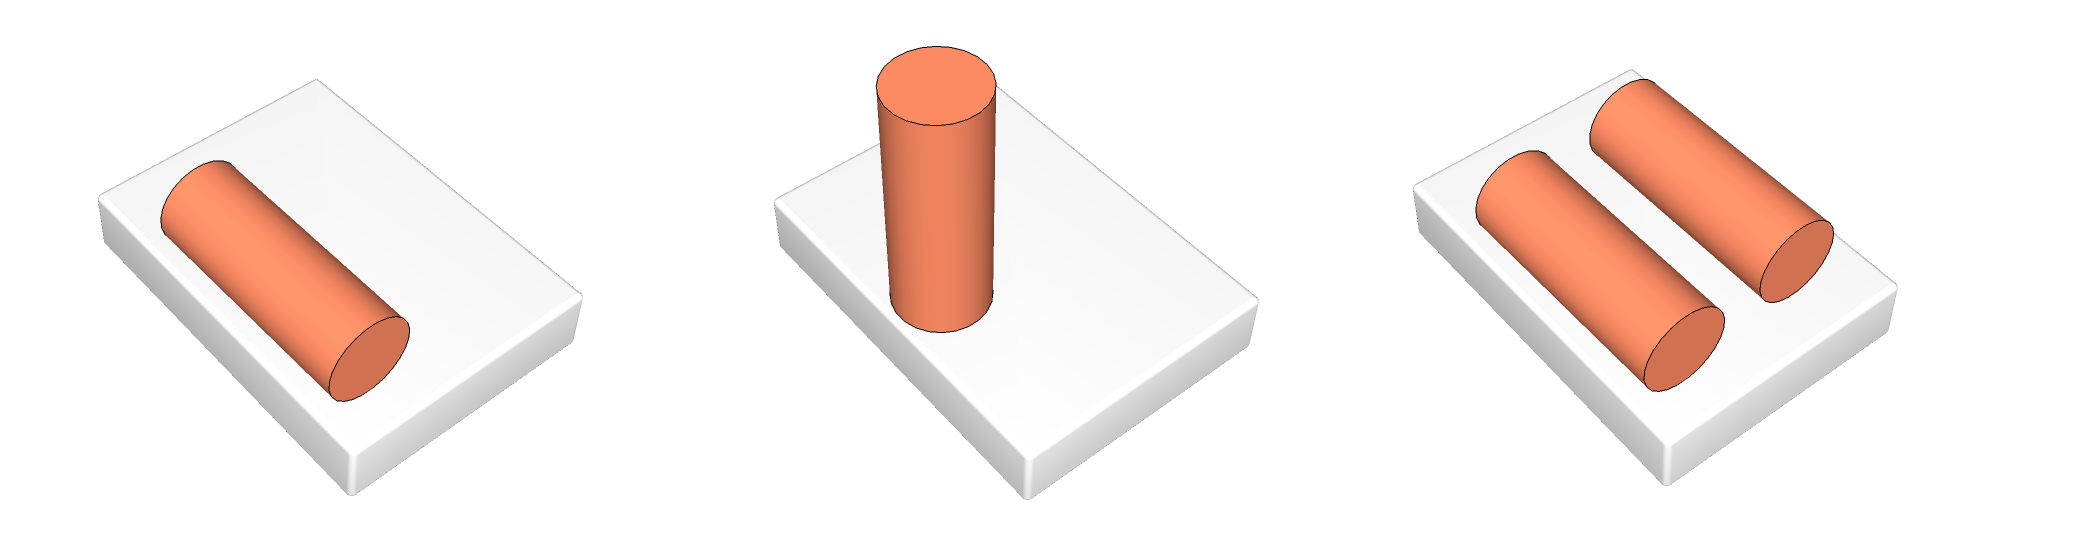
\includegraphics[width=0.8\textwidth]{images/prot_model_bed}
\captionof{figure}{Cylindrical human body model and various poses on mattress \cite{braun2012context}}
\label{fig:prot_model_bed}
\end{minipage}

To identify occupation and positioning we use a very simple model for estimating the effect of a human body on the sensor values. As previously mentioned, the sensors react to both presence of a body and applied pressure. The human body is modeled as a cylindrical object on the mattress. The object can be either sitting or lying and there might be multiple on a single bed. A few potential poses are shown in Figure \ref{fig:prot_model_bed}. It is assumed that a sitting person will cause a high pressure within a small region and that a lying person has a moderate pressure distributed over a larger area. Thus, the challenge of determining posture and orientation from a limited number of capacitive sensors, tuned to detect pressure, can be formulated as an inverse problem. If we assume a constant density of the cylinder and a uniformly deforming mattress, the idealized pressure distribution is uniform as shown in Figure \ref{fig:prot_model_pressure}.

\begin{minipage}{\linewidth}
\centering
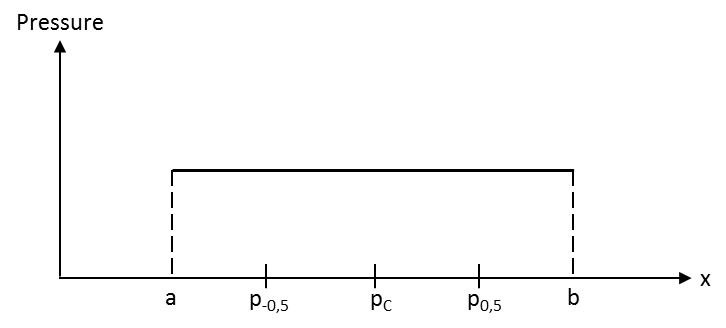
\includegraphics[width=0.6\textwidth]{images/prot_model_pressure}
\captionof{figure}{Pressure distribution of a uniform cylinder \cite{braun2012context}}
\label{fig:prot_model_pressure}
\end{minipage}

The system is further simplified by reducing the significant values of the pressure distribution to just two distinct values. Be $p_c$ is the center of pressure and $p_{-0.5}$, $p_{0.5}$ the points enclosing half of the pressure distribution. The center of pressure and standard deviation $\sigma$ are sufficient to describe the system, as shown in the following equations:

\begin{align}
p_c&=\frac{a+b}{2} & \sigma&=\sqrt{\frac{(b-a)^2}{12}}
\end{align}
\begin{align}
p_{-0.5}&=p_c-\sigma &	p_{0.5}&=p_C+\sigma
\end{align}

The raw data from the sensor is considered as random, uniform sampling, a discretization of the continuous distribution. The center of pressure and the standard deviation are calculated using the geometric information, the position of the sensor $\overrightarrow{x}$.
\begin{equation}
p_c=\frac{\sum_{i=1}^n{v_i\overrightarrow{x}}}{\sum_{i=1}^n{v_i}}
\end{equation}
\begin{equation}
\sigma=\sqrt{\frac{1}{n}(\sum_{i=1}^n{\overrightarrow{x}^2}-\frac{1}{n}(\sum_{i=1}^n{\overrightarrow{x}})^2}
\end{equation}

Using this model a set of potential poses cover the most common situations has been determined. Potential poses for one and two occupants are distinguished. One person may sit at a certain location or lie on the bed in various angles. It is assumed that the head is always at the upper part of the bed. Two persons may either both sit, both lie down, or one is sitting while the other is lying. 
The limitations of this model concerning the actual system are the non-uniform pressure propagation throughout the mattress, as well as the non-linear sensor response on different pressure levels. Therefore, it is not expected that the deviations adhere to the theoretical model, but instead configurable thresholds are used that allow for increased robustness in exchange for precision.

\begin{minipage}{\linewidth}
\centering
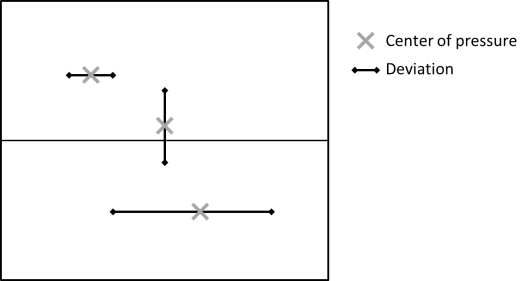
\includegraphics[width=0.7\textwidth]{images/smartbed_cog}
\captionof{figure}{Calculating centers of pressures and deviation \cite{braun2012context}}
\label{fig:smartbed_cog}
\end{minipage}

Occupation and posture detection are performed by dividing the two person bed into a left and right section. For each side the total sensor values, assumed center of pressure using weighted average and the standard deviation are calculated individually(Figure \ref{fig:smartbed_cog}). The same calculation is performed between the two areas, allowing to distinguish the specific side of activity or detecting persons that are lying on the bed diagonally.
Using these six intermediate values it is possible to map the different poses. If all activity is on one side and the horizontal deviation is low, it can be assumed that one person is sitting. Additionally, the intermediate values can be used to gather more information, e.g. the exact location a person is sitting at. 

\subsubsection{Multi-body models}
If it necessary to identify more complex human behaviors than sitting and lying, a single body model is no longer sufficient. In the briefly mentioned work by Harada et al. the underlying model was a 3D representation of an average human body that could move various joints freely \cite{harada2000human}. This allows to detect a variety of different postures, in this case using an iterative process based on potential energy, momentum and difference between the actual and simulated pressure distribution. Using such full body models, based on an internal skeleton of connected joints is also common in full body gesture tracking systems. However, while in those cases the volume of the different body parts is important, there is not necessarily any additional physical simulation of properties, such as weight and density \cite{Shotton2013}. 

In a project together with student Sebastian Frank, a concept for a smart chair was developed that unobtrusively integrates a set of capacitive proximity sensors to detect presence, posture, activity and breathing rate of a person sitting on the chair \cite{Braun2013ChairAid}. By placing suitably sized electrodes strategically, at locations that allow getting a good measure of the most significant body parts. Using eight electrodes distributed between seat, backrest and armrests it the sensor values are mapped to postures using two different methods, according to the specific purpose of the underlying application. The first method directly translates the sensor values to body part positions, while the second uses a machine learning classification.

\subsubsection*{Direct manipulation of skeleton model}
\begin{minipage}{\linewidth}
\centering
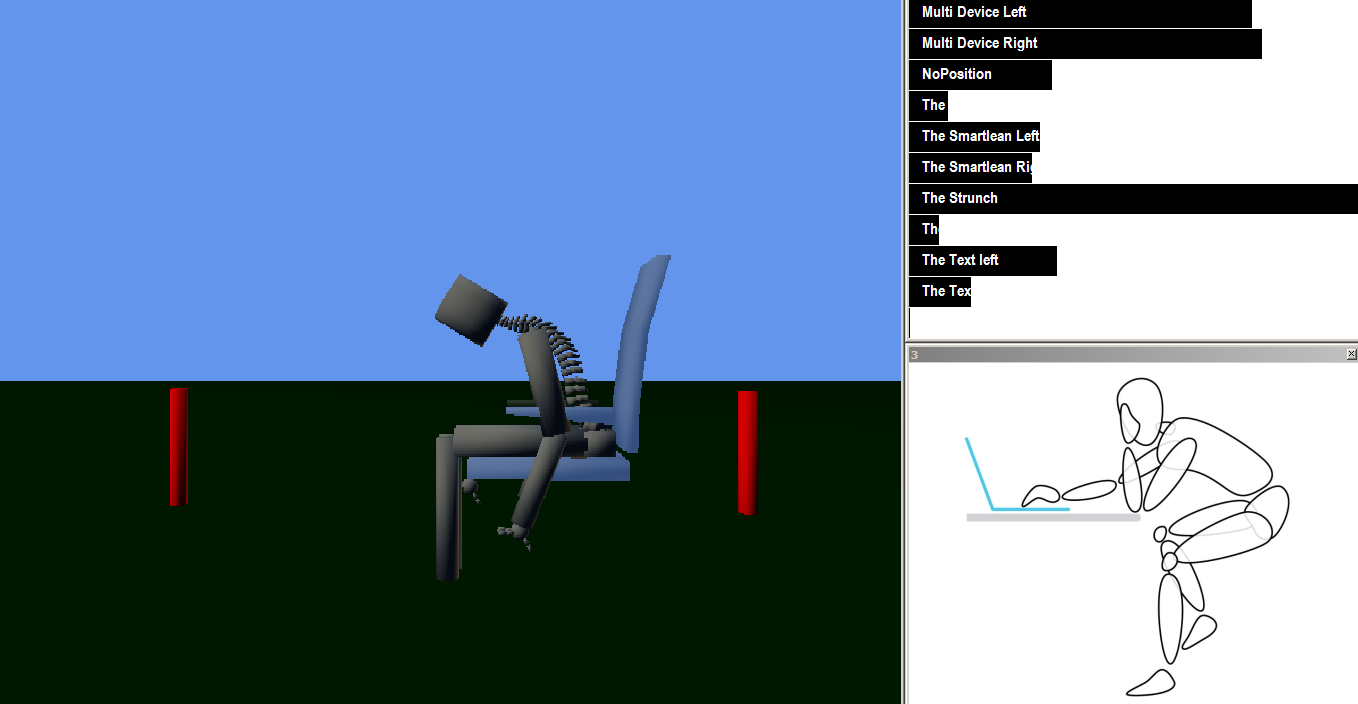
\includegraphics[width=0.7\textwidth]{images/smartchair_software}
\captionof{figure}{Screenshot of the Capacitive Chair application showing the fitted 3D model on the left, posture detection on the upper right and the recognized posture on the lower right}
\label{fig:smartchair_skeleton_model}
\end{minipage}

In Figure \ref{fig:smartchair_skeleton_model} the skeleton model can be seen. The skeleton model is comprised of 36 bones that are in 15 different groups. As those are combined to each other the degrees of freedom are significantly reduced to just 10. Sensors close to the different body parts will modify the associated parts of the model. As an example, the distance of the left lower arm group is determined by the sensor in the left armrest. However, as the groups are connected, this will also modify the orientation of the left upper arm. Accordingly, if the sensor behind in the lower backrest detects a receding lower back, the position and orientation of the other back groups, head and arms are also modified. Thus, the fitting method attempts to place the different groups of the model according to current sensor readings. A collection of rules is used that follows the flowchart outlined in Figure \ref{fig:capchair_flow}.

\begin{minipage}{\linewidth}
\centering
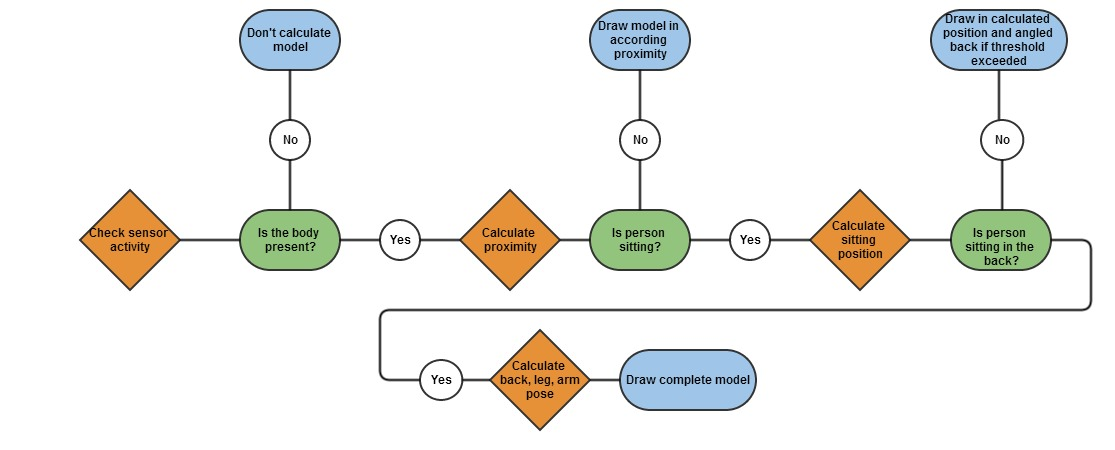
\includegraphics[width=0.9\textwidth]{images/capchair_flow}
\captionof{figure}{Flowchart of the model fitting process of the grouped skeleton parts and performed calculations}
\label{fig:capchair_flow}
\end{minipage}

The calculation of the different steps varies and is outlined shortly in the following enumeration:
\begin{enumerate}
\item \emph{Check sensor activity} uses a threshold of the different sensors to determine the presence of any objects in detection distance
\item \emph{Calculate proximity} use a second thresholds of seat sensors to determine sitting or non-sitting status
\item \emph{Calculate sitting position} use a weighted average of the seat area sensors to determine position on seat
\item \emph{Calculate back, leg, arm pose} calculate back pose by determining distance from back to backrest based on sensor values. Raise leg according to proximity to front seat sensor. Calculate arms based on proximity to arm rests.
\end{enumerate}

This method allows a fine-grained fitting of the model to the sensor values that closely resembles the pictures of a person moving in the chair. A number of poses and the accordingly fitted 3D models using this method can be seen in Figure \ref{fig:smartchair_skeleton_poses}.

Using a fitting method that allows to detect fine movements enables a number of unique applications. One example is to track a set of different exercises that can be performed on an office chair, in order to prevent future back problems. Following an exercise routine can significantly reduce the indicative risks \cite{robertson2009effects}. Some of the common exercises can be tracked for accuracy and number of repetitions using the capacitive proximity sensors in the chair.

\begin{minipage}{\linewidth}
\centering

\includegraphics[width=0.7\textwidth]{images/placeholder}
\captionof{figure}{Screenshot of the Capacitive Chair application showing the fitted 3D model on the left, posture detection on the upper right and the recognized posture on the lower right}
\label{fig:smartchair_skeleton_poses}
\end{minipage}

A limitation of the above method are the fixed threshold levels that are set based on experience. Either a calibration method can be used that personalizes the different thresholds, or another form of classifications that is based on training with a larger variety of different body volumes. It is suitable to use machine learning methods for this task, as they are designed to learn from a larger set of training data and provide numerous classification methods. However, this leads only to a discrete set of different postures, limiting some potential applications. One potential method is described in the following section.

\subsubsection*{SVM classification}
\begin{minipage}{\linewidth}
\centering

\includegraphics[width=0.7\textwidth]{images/placeholder}
\captionof{figure}{Screenshot of the Capacitive Chair application showing the fitted 3D model on the left, posture detection on the upper right and the recognized posture on the lower right}
\label{fig:smartchair_gps_poses}
\end{minipage}

Support vector machines (SVM) are a supervised learning method that is primarily used for linear classification of n-dimensional features \cite{hearst1998support}. They are clustering data by calculating a hyperplane from training data that maximizes the distance from the closest features. A fast learning method is using sequential minimal optimization and was proposed by Platt \cite{platt1999fast}. The algorithm requires normalized values. A dynamic normalization algorithm constantly analyzes the sensor data for minimum and maximum values and accordingly calculates the normalized value. There is a variety of different software frameworks for machine learning that support training and recall of SVMs, thus there is no need for reimplementing these methods. As there is an implicit weighting of features according to significance, there is no need to pre-process or weigh the sensor data.

The training data is collected from a set of persons that have a significant variance in body shapes in both height and girth. SVMs support an arbitrary number of different groups for classification. However, the number of significant poses on a chair is limited. The Global Posture Study by office furniture manufacturer Steelcase Inc. analyzes the most common poses with a focus on information consumption from modern technical devices, such as smart phones or tablets \cite{globalPosture}. The different postures are shown in Figure \ref{fig:smartchair_gps_poses}. A capacitive office chair should be able to distinguish most of these poses if training data has been collected from a large enough number of suitable candidates. Additionally, using sensors clearly positioned on a certain side of the chair, e.g. the armrest sensors, it is possible to associate directional varieties of the asymmetric postures.